\documentclass[a4paper,
               % boxit,        % check whether paper is inside correct margins
               biblatex,       % biblatex is used
               keeplastbox,    % flushend option: not to un-indent last line in References
               % nospread,     % flushend option: do not fill with whitespace to balance columns
               % hyphens,      % allow \url to hyphenate at "-" (hyphens)
               % xetex,        % use XeLaTeX to process the file
               % luatex,       % use LuaLaTeX to process the file
               ]{jacow-2_1}    % uses jacow-2_1 to better support BibLaTeX
               
%
% CHANGE SEQUENCE OF GRAPHICS EXTENSION TO BE EMBEDDED
% ----------------------------------------------------
% test for XeTeX where the sequence is by default eps-> pdf, jpg, png, pdf, ...
%    and the JACoW template provides JACpic2v3.eps and JACpic2v3.jpg which
%    might generates errors, therefore PNG and JPG first
%
\makeatletter%
	\ifboolexpr{bool{xetex}}
	 {\renewcommand{\Gin@extensions}{.pdf,%
	                    .png,.jpg,.bmp,.pict,.tif,.psd,.mac,.sga,.tga,.gif,%
	                    .eps,.ps,%
	                    }}{}
\makeatother

% CHECK FOR XeTeX/LuaTeX BEFORE DEFINING AN INPUT ENCODING
% --------------------------------------------------------
%   utf8  is default for XeTeX/LuaTeX 
%   utf8  in LaTeX only realises a small portion of codes
%
\ifboolexpr{bool{xetex} or bool{luatex}} % test for XeTeX/LuaTeX
 {}                                      % input encoding is utf8 by default
 {\usepackage[utf8]{inputenc}}           % switch to utf8

\usepackage[USenglish]{babel}			 

\usepackage[final]{pdfpages}
\usepackage{multirow}
\usepackage{ragged2e}
 
\addbibresource{ska-status-icalepcs2017.bib}

%
% command for typesetting a \section like word
%
\newcommand\SEC[1]{\textbf{\uppercase{#1}}}

%%
%%   Lengths for the spaces in the title
%%   \setlength\titleblockstartskip{..}  %before title, default 3pt
%%   \setlength\titleblockmiddleskip{..} %between title + author, default 1em
%%   \setlength\titleblockendskip{..}    %afterauthor, default 1em

%\copyrightspace %default 1cm. arbitrary size with e.g. \copyrightspace[2cm]

% testing to fill the copyright space
%\usepackage{eso-pic}
%\AddToShipoutPictureFG*{\AtTextLowerLeft{\textcolor{red}{COPYRIGHTSPACE}}}


\begin{document}

\title{Status of the Square Kilometre Array}

\author{
	J. Santander-Vela\thanks{j.santander-vela@skatelescope.org},\\
	representing the SKA Organisation, Macclesfield, United Kingdom
}
	
\maketitle

%2345678901234567890123456789012345678901234567890123456789012345678901-
\begin{abstract}
	The Square Kilometre Array (SKA) is a international project to build a number of multi-purpose radio telescopes, operating as a single observatory, that will play a major role in answering key questions in modern astrophysics and cosmology. It will be one of a small number of cornerstone observatories around the world that will provide astrophysicists and cosmologists with a transformational view of the Universe. Two major goals of the SKA is to study the history and role of neutral Hydrogen in the Universe from the dark ages to the present-day, and to employ pulsars as probes of fundamental physics. Since 2008, the global radio astronomy community has been engaged in the development of the SKA and is now nearing the end of the \emph{Pre-Construction} phase. This talk provides an overview of the current status of the SKA and the plans for construction, focusing on the computing and software aspects of the project.
\end{abstract}


\section{Introduction} % (fold)
\label{sec:introduction}
The Square Kilometre Array (SKA) is an international project that has the aim of building multi-purposes radio telescopes, with an equivalent collecting area of at least one square kilometre, and thus unprecedented sensitivity, so that key questions in modern astrophysics and cosmology can be answered.

The original SKA Science book was published in 2004~\cite{2004NewAR..48..979C}. In 2015, \citetitle{2015aska.confE.....}~\cite{2015aska.confE.....} was published with an update to the SKA science book after a decade of development of the SKA concept, incorporating more than 130 scientific use cases that will be possible thanks to the SKA telescopes.

Those science cases cover Galaxy Evolution, Cosmology and Dark Energy\footnote{http://skatelescope.org/galaxyevolution/}~\cite{2015aska.confE..67P, 2015aska.confE..16M, 2015aska.confE..51F}, Strong-Field Tests of Gravity\footnote{http://skatelescope.org/gravity-einstein-pulsars/}~\cite{2015aska.confE..36K}, Cosmic Magnetism\footnote{http://skatelescope.org/magnetism/}~\cite{2015aska.confE..92J}, The Cosmic Dawn and the Epoch of Reionisation\footnote{http://skatelescope.org/cosmicdawn/} ~\cite{2015aska.confE...1K}, and research on the Cradle of Life\footnote{http://skatelescope.org/cradle-life/}~\cite{2015aska.confE.115H}. The amount of physical disciplines foreseen to be encompassed by the SKA telescopes is one of the largest for any ground based facility to date.

The SKA project is currently in what is known as SKA Phase 1, or SKA1, in which two telescopes approximately with 10\% of the target collecting area are being built, namely SKA1-Mid, and SKA1-Low, in order to prove the feasibility of the techniques and derisk the construction of the next phase of the project, SKA Phase 2, or SKA2.

The goal is to have a single observatory entity, that will construct and operate two SKA1 telescopes (SKA1-Mid and SKA1-Low), with presence in three sites: Australia (SKA1-Low), South Africa (SKA1-Mid), and United Kingdom (Headquarters and central operations).

This talk focuses on the progress and status of the SKA1 telescopes. It starts by describing the SKA Organisation itself (Sec.~\ref{sec:ska_organisation}), the current SKA timeline (Sec.~\ref{sec:ska1_timeline}), and the overall project organisation (Sec.~\ref{}). 

% section introduction (end)

\section{SKA Organisation} % (fold)
\label{sec:ska_organisation}
The organisation overseing the SKA1 project is the SKA Organisation (SKAO), currently a limited liability non-for-profit company registered in England and Wales.

The SKAO is in the process of the becoming an Inter-Govermental treaty Organisation (IGO), not unlike the European Southern Observatory (ESO) or the European Council for Nuclear Research (CERN). The timeline for that process will be detailed in Sec.~\ref{sec:ska1_timeline}.

Currently\footnote{https://skatelescope.org/participating-countries/} there are ten countries that are Full Members of the SKAO (listed in alfabetical order): Australia, Canada, China, India, Italy, New Zealand, South Africa, Sweden, The Netherlands, and United Kingdom. Other countries are involved in the design of the SKA1 telescopes, and it is estimated that \~20 countries and more than 100 organisations are contributed to that effort.

SKAO's headquartes are located within the boundaries of the Jodrell Bank Observatory, in the middle of the Cheshire plain, under direct view of the 70m Lovell Telescope.

As part of the UK commitment as host country for the SKAO HQ, and the IGO, an expansion to the HQ is being constructed with the intention of becoming a nexus for radio astronomy. An artist rendition of the new building can be found in Fig.~\ref{fig:SKA-HQ-render}, while the current status of the work, as of September 2017, can be seen in Fig.~\ref{fig:SKA-HQ2-aerial}.

\begin{figure}[!htb]
  \centering
    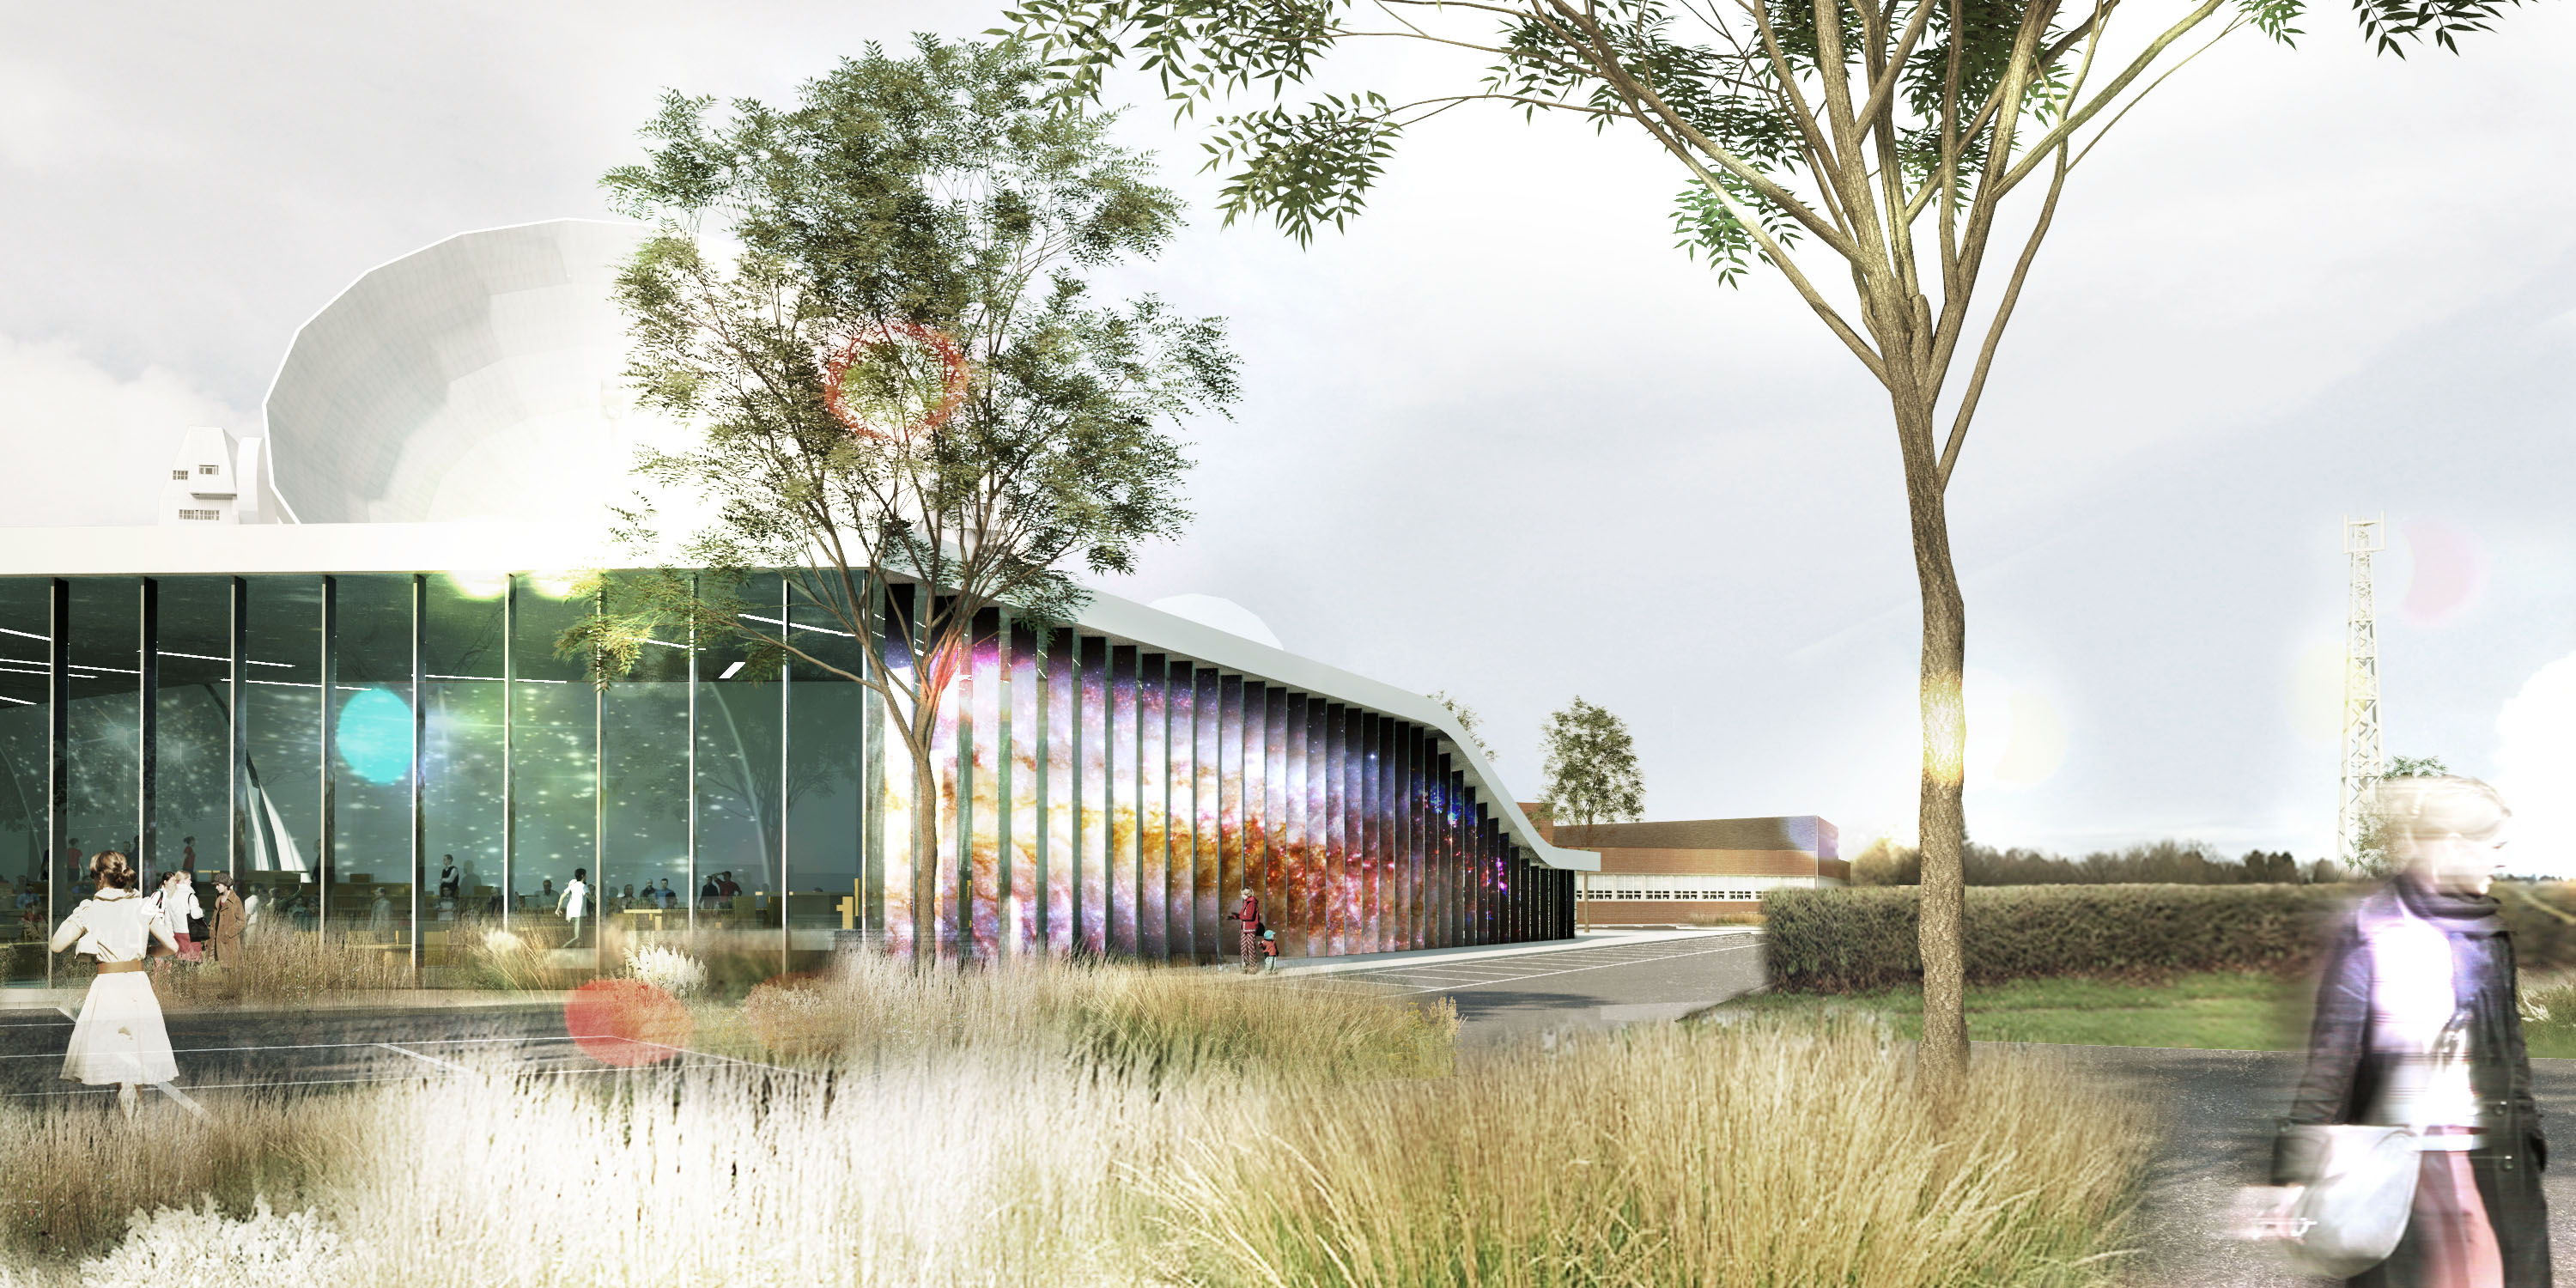
\includegraphics[width=\columnwidth]{figs/SKA-HQ-render}
  \caption{Artist's view of the future SKAO HQ2, with the Council chamber in the foreground, and the Lovell telescope current Jodrell Bank Observatory building in the background.}
  \label{fig:SKA-HQ-render}
\end{figure}

\begin{figure}[!htb]
  \centering
    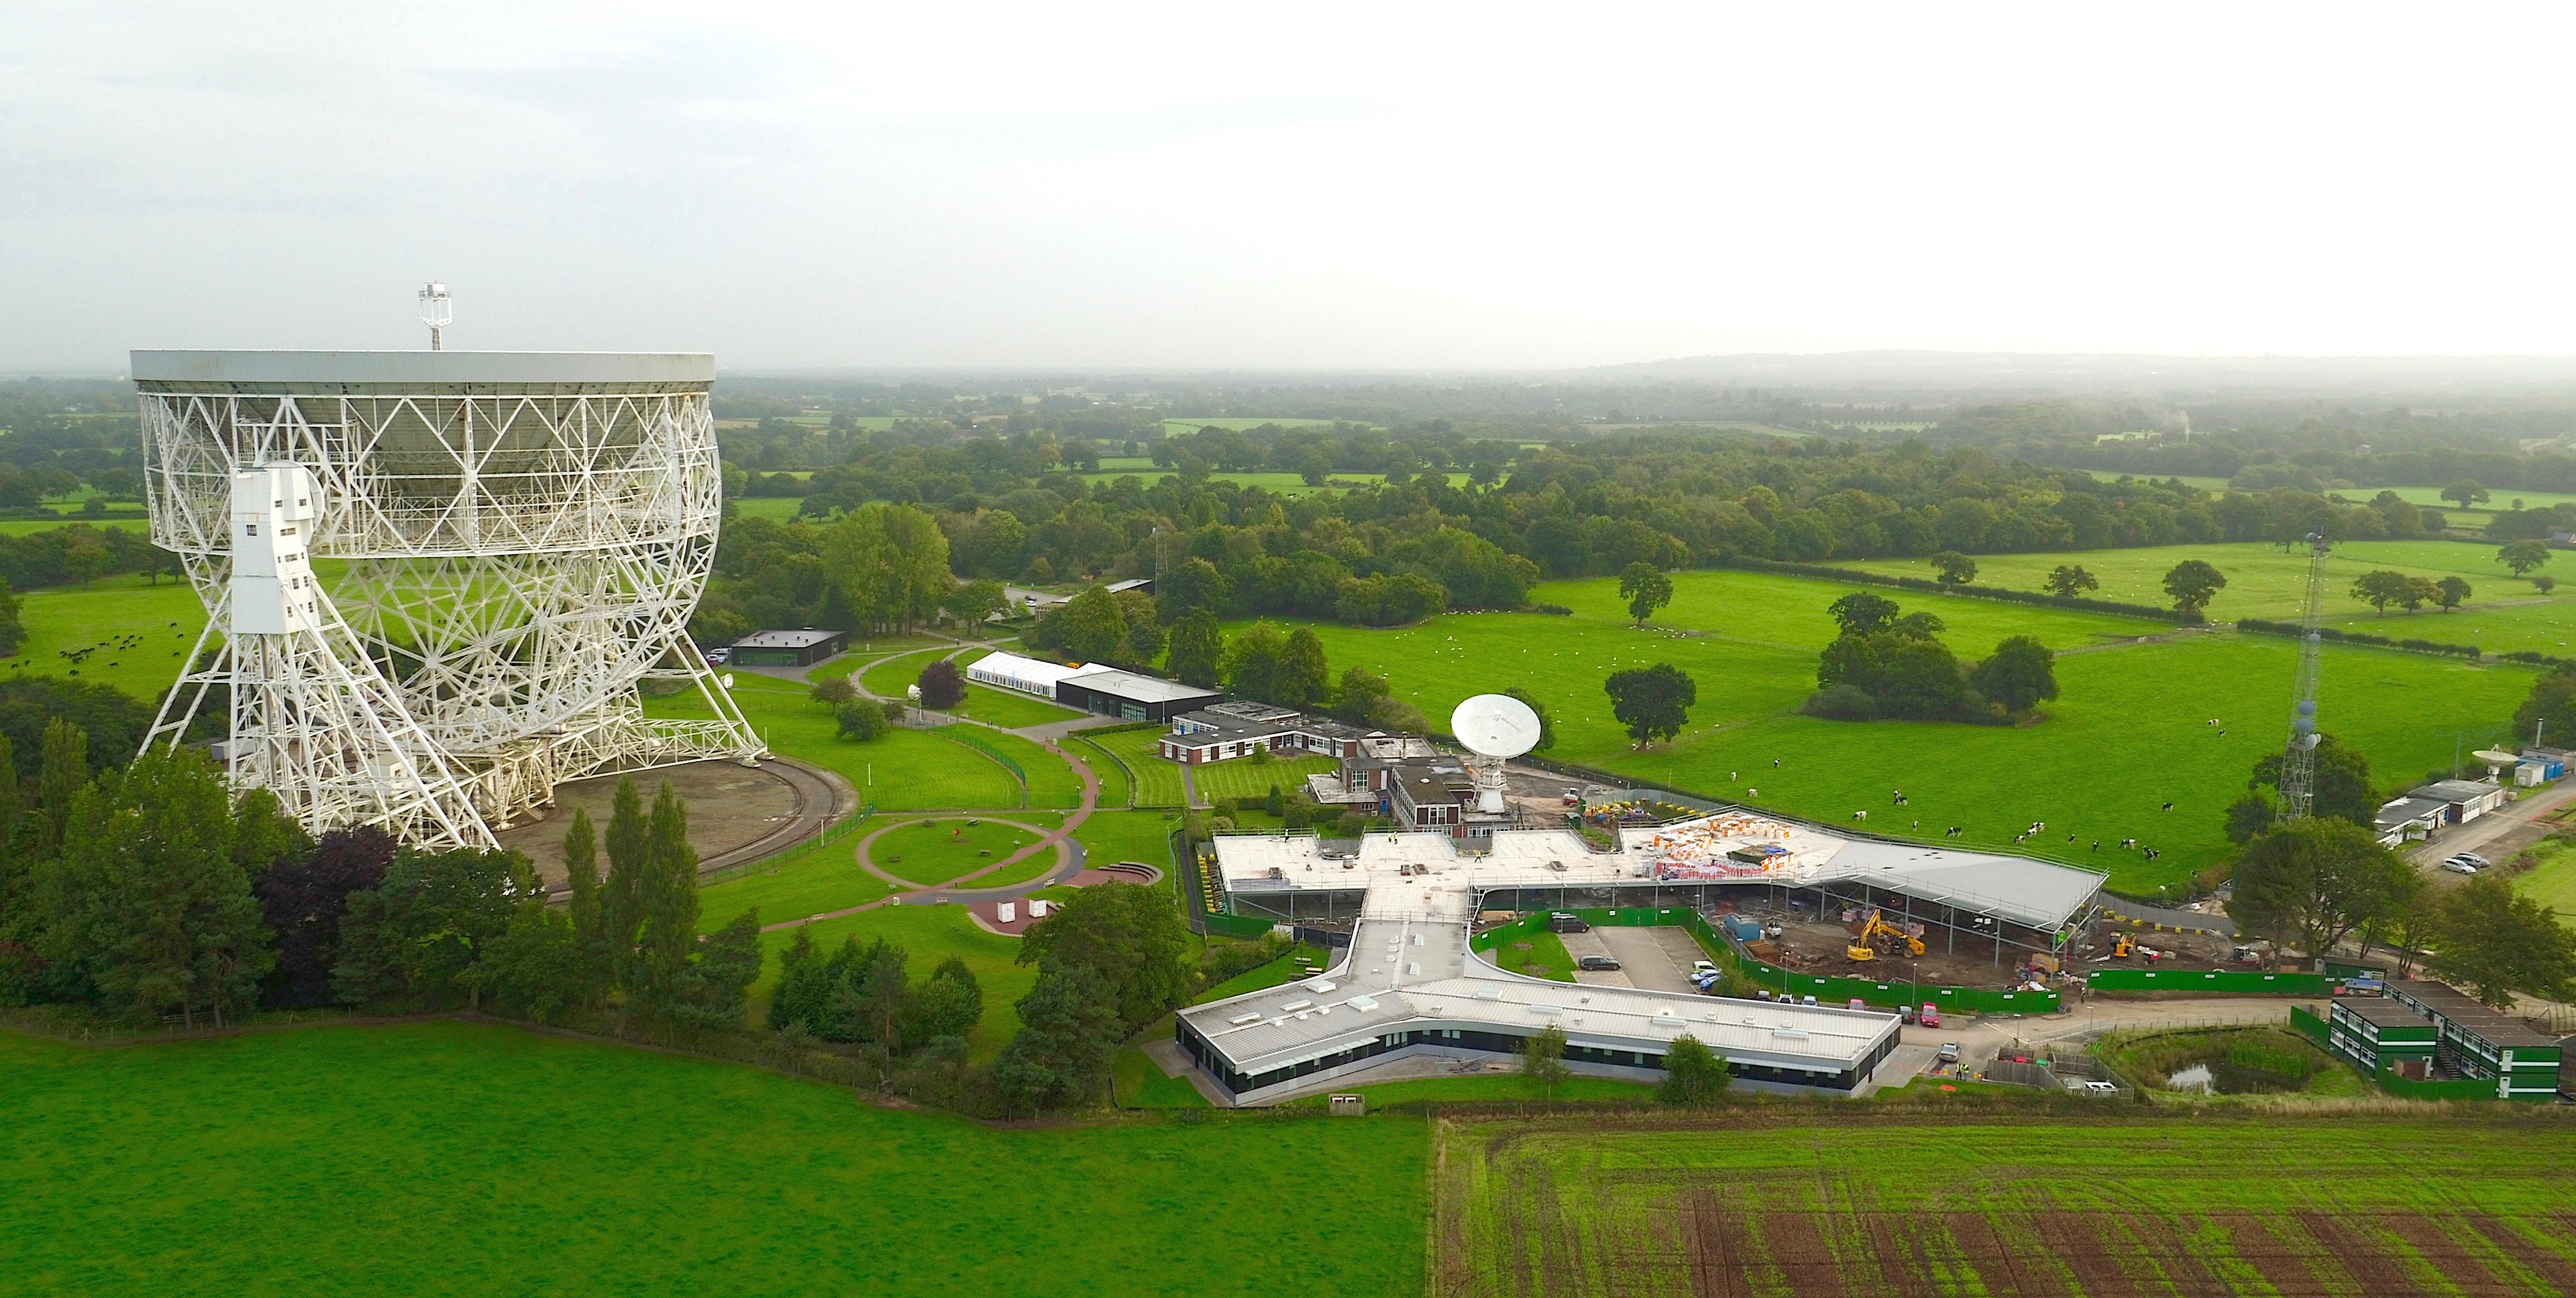
\includegraphics[width=\columnwidth]{figs/SKA-HQ2-aerial}
  \caption{Aerial view of the current status of the SKAO HQ2 building, after the steel structure has been erected, and concrete slabs installed. The current SKAO HQ is in the foreground, Council chamber can be seen raising to the right.}
  \label{fig:SKA-HQ2-aerial}
\end{figure}

% section ska_organisation (end)

\section{SKA1 Telescopes} % (fold)
\label{sec:ska1_telescopes}

As previously indicated, in this Phase 1 (SKA1) we intend to build two telescopes, SKA1-Mid, and SKA1-Low, within a cost cap for both telescopes of 674~MEur (2016 value).

The SKA1-Low will be located in Western Australia, within the Murchison Radio-astronomy Observatory (MRO), which defines a Radio Quiet Zone for the benefit of the SKA1-Low, but also the Australian SKA Pathfinder (ASKAP) and Murchison Widefield Array (MWA) precursor telescopes. Fig.~\ref{fig:figs_SKA1-Low_locations} shows where the MRO is located, together with the positions of Geraldton (the designated Engineering Operations Centre), and of the Pawsey Supercomputing Centre, currently the designated host for the Science Processing Facility.

SKA1-Low will consist of 131,072 log-frequency, dual polarisation dipole antennas, organised in 512 stations of 256 antennas each. 

\begin{figure}[!htb]
  \centering
    \includegraphics[width=\columnwidth]{figs/SKA1-Low_locations.pdf}
  \caption{Relevant locations of SKA1-Low in Western Australia. The image shows the location of the Murchison Radio-astronomy Observatory,  the Engineering Operations Centre in Geraldton, and the Pawsey Supercomputing Centre, where we expect the Science Data Processor for SKA1-Low to be located.}
  \label{fig:figs_SKA1-Low_locations}
\end{figure}

\cite{SKA-TEL-SKO-0000002_v3} defines the baseline 
design capabilities of the SKA1-Mid and SKA1-Low telescopes.


% section baseline_design (end)

\section{SKA1 Consortia} % (fold)
\label{sec:ska1_consortia}
TBD.

% section ska1_consortia (end)

\section{SKA1 Timeline} % (fold)
\label{sec:ska1_timeline}
TBD.
 
% section ska1_timeline (end)

\section{SKA1 Control Hierarchy and Control System Guidelines} % (fold)
\label{sec:ska1_control_hierarchy_and_control_system_guidelines}

% section ska1_control_hierarchy_and_control_system_guidelines (end)

\section{SKA1 Central and Science Data Processing} % (fold)
\label{sec:ska1_central_and_science_data_processing}

Challenge of processing, storage.

CERN-SKA agreement on extreme-scale computing\footnote{http://skatelescope.org/news/ska-signs-big-data-cooperation-agreement-cern/}.

% section ska1_central_and_science_data_processing (end)

\section{Conclusion} % (fold)
\label{sec:conclusion}
TBD. Any conclusions should be in a separate section directly preceding
the \SEC{Acknowledgement}, \SEC{Appendix}, or \SEC{References} sections, in that
order.

% section conclusion (end)

\section{Acknowledgement} % (fold)
\label{sec:acknowledgement}
TBD. Any acknowledgement should be in a separate section directly preceding
the \SEC{References} or \SEC{Appendix} section.

% section acknowledgement (end)

\section{Appendix} % (fold)
\label{sec:appendix}
TBD. Any appendix should be in a separate section directly preceding
the \SEC{References} section. If there is no \SEC{References} section,
this should be the last section of the paper.

% section appendix (end)


%\section*{References} % (fold)
\label{sec:references}
\printbibliography

% section references (end)




\end{document}
